\section{Very wide focus (Theorem~\ref{thm:verywide})}
\label{sec:verywide}

Theorem~\ref{thm:verywide} was reduced in Sec.~\ref{sec:main} to Proposition~\ref{prop:BE} (where $\tau\ge\tau_0(\ell)=4\ln\ell+40$) and Lemma~\ref{lem:P} (everywhere).
This section proves both.
It uses neither the lines nor the brightness hypothesis.

\subsection{Proposition~\ref{prop:BE}: what changes in Lemma~BE}

Lemma~BE of~\cite{H} (\Hsec{VII}) proves $(a)+(a')\ge1.1\times10^{-5}/\sigma$ for $B\le10^4$ and $\sigma\ge10^{-3000}$ ($\ell\le6907.8$).
Its proof uses these two limits in four places only:
the numerical lower bound of $1-e$;
the comparison $\sigma^2\Jww>0.6\sigma^2\ge6\times10^{-5}b$ in the case $L^2<1$;
the value $U_1\le29.4$ of the window constant;
and the comparison of every remainder with $\sigma^2\Jww\ge0.6\sigma^3$, which needs $\tau\ge5\times10^7$.
The core of the proof, the mean-square bound of the cross term (steps BE-a to BE-3 of~\cite{H}), depends neither on $B$ nor on $\ell$.
We keep that core and change three things:
$1-e\ge y/(2+y)$ is used for general $B$;
the remainders are written as $\sigma^2$ times a ratio free of $\sigma$ and compared with the main term of each case;
and the remainder $a_4^*$ of Lemma~A4* of~\cite{H} is written as a multiple of $(1-e)W$.
Lemma~20 of~\cite{F} (narrow envelopes have $\tau>80$) is not used: $\tau\ge\tau_0(\ell)$ is a hypothesis, and Lemmas~19, 21--23 of~\cite{F} are used at that $\tau$ directly; their statements do not assume a size of $\tau$, and their remainders are written through $\nu_k(\tau,\beta)$.
Paper~H uses Lemma~R and Lemma~A4* in the same way at $\tau\ge20$.

\subsection{Proof of Proposition~\ref{prop:BE}}

Notation of~\cite{F,H}: $y=(1-b)^2/(2B)$, $e=e^{-y/2}$, $\beta=(1-b)\sqrt{\tau/(2B)}$, $\nu_k=2\sum_{n\ge1}n^ke^{-n^2\tau/2}e^{n\beta}$, $z=\Qb\nu_0/2$, $J=\sigma^2\Jww$, $\mathrm{den}=b+W+J$; $x=\tau B\sigma^2$ and $b=B\sigma^2$.

\emph{(0)} $\tau B=x/\sigma^2\ge5\times10^{11}$, hence $1/B\le\tau/(5\times10^{11})$ and $\beta\le10^{-6}\tau$.

\begin{lemma}[$\nu_k$ at moderate $\tau$] \proofst
\label{lem:nu}
If $\tau\ge60$, $\beta\le10^{-6}\tau$ and $k\le4$, then $\nu_k\le\bar\nu(\tau)=2.0000001\,e^{-0.499999\tau}$.
\end{lemma}
\begin{proof}
The ratio of the $n$-th to the first term is at most $n^4e^{-0.499999(n^2-1)\tau}$, and $\sum_{n\ge2}n^4e^{-0.499999(n^2-1)\tau}\le1.32\times10^{-38}$ for $\tau\ge60$. The first term is at most $2e^{-0.499999\tau}$.
\end{proof}

\emph{(2) The cross term (as in~\cite{H}).}
Replacing the term $-\sigma^2\gamma_P\Phi/(1-z)$ of Lemma~23 of~\cite{F} by the mean-square step with $c=(b+J)/(16\sigma^2)$ and $\Lambda=10^{-3}/\sigma^2$, the $\Phi$-part is at most $b\Psi/2+J/4$, and the curvature part is at most $\rho_W(1-e)W_{\rm per}$ plus a tail, with
\begin{gather}
\rho_W=\frac{48(1+\Qb)K_1\sigma^2}{(1-b)^2},\nonumber\\ K_1\sigma^2=\frac{10^{-3}}{1-\Qb}+\frac{\sigma^2(U_1^2+\frac12)}{(1-\Qb)^3},
\end{gather}
and $\rho_W\le0.0801$ for $\ell\ge960.8$ and $b\le(8\ell+100)\sigma^2$.
No size of $B$ is used here: the cross term costs $8\%$ of the ripple information whatever the width of the focus.

\emph{(3) $a_4^*$ as a multiple of $(1-e)W$.}
With $e\beta^2/(1-e)\le2\tau$, $e\beta/(1-e)\le2\sqrt{2\tau B}/(1-b)$ and the window constant $U_1$,
\begin{gather}
a_4^*\le\delta_4(1-e)W_{\rm per},\nonumber\\ \delta_4=\tfrac53\bigl[\tau\bar\nu+2\sqrt{2\tau B}\,\bar\nu\,\sigma\Xi/(1-b)\bigr],\nonumber\\ \Xi=\frac{U_1+\Qb e^{-1/2}}{\sqrt2(1-\Qb)}+\frac1{2\sqrt\pi}.
\end{gather}

\emph{(4) The collected inequality.}
With the sandwich $W_{\rm per}\le((1+z)W+\tfrac12b\tau\Qb\nu_2)/(1-\nu_0)$ of Lemma~22 of~\cite{F},
\begin{equation}
\begin{aligned}
2N_\phi\ \ge\ &(1-e)W\,c_1+b\Psi\,c_2-\frac J{4(1-z)}-\mathrm{rem}-(\text{tail}),\\
c_1=&\,1-\frac{\sigma^2}{(1-e)(1-\bar\nu)}-\frac{(\rho_W+\delta_4)(1+z)}{(1-z)(1-\bar\nu)},\\ c_2=&\,\frac1{1+z}-\frac1{2(1-z)},
\end{aligned}
\end{equation}
where rem is the sum of eleven remainders: $a_1,a_2,a_3,a_5,\ldots,a_{10}$ from the proof of Lemma~23 of~\cite{F}, the term proportional to $\Phi$ in its statement (with $\Phi\le2$), and the part proportional to $b$ that the sandwich brings into $\rho_W$ and $\delta_4$.
The only difference from the collected inequality of~\cite{H} is that $\delta_4$ sits in $c_1$.

\emph{(5) The remainders free of $\sigma$.}
With $x=\tau B\sigma^2$, $\sqrt x=\sigma\sqrt{\tau B}$, $b=B\sigma^2$ and $\sqrt xN_1\le U_1$, each remainder is $\sigma^2$ times a term $T_i=K_iB^{a_i}$, $a_i\in\{0,\tfrac12,1\}$, with $K_i$ a function of $\tau$ and $\ell$ (App.~\ref{app:D} lists all eleven, separated by origin).
The largest is $a_6=\nu_1(xN_1\sigma c_\chi+\sigma\sqrt x(1+\Qb)\gamma_P/\sqrt2)$, which becomes $\sqrt{\tau B}(U_1c_\chi+(1+\Qb)\gamma_P/\sqrt2)\bar\nu$; at $\ell=960.8$, $\tau=\tau_0$, $B=8\ell+100$ it is $4.12\times10^{-9}$.

\begin{lemma}[remainders] \status{proof; values checked in interval arithmetic}
\label{lem:R}
Let $\ell\ge960.8$ and $\tau\ge\tau_0(\ell)$, and let $S_R=\sum_iT_i$.
(R-2) For $0<B\le8\ell+100$: $S_R/(1-z)\le\rho_2=4.76\times10^{-9}$.
(R-1) $\mathrm{rem}/b=S_R/(B(1-z))\le\rho_1=5.49\times10^{-11}$.
\end{lemma}
\begin{proof}
Put $\bar B=8\ell+100$.
\emph{In $B$.} $B$ enters $K_i$ only through $\rho_W$ and $\delta_4$, which increase with $B$. So every $T_i$ is non-decreasing in $B$, and (R-2) is largest at $B=\bar B$. For (R-1), first bound $\rho_W$ and $\delta_4$ by their values at $\bar B$; call the result $\bar K_i$. The remaining powers of $B$ are $B^{-1}$, $B^{-1/2}$ and $1$, and $1/B\le M(\tau)=1+\tau/(5\times10^{11})$ (by (0) if $B<1$). Hence $S_R/B\le M\sum_{a_i=0}\bar K_i+\sqrt M\sum_{a_i=1/2}\bar K_i+\sum_{a_i=1}\bar K_i$.
\emph{In $\tau$.} Each term is a constant times $\tau^j\bar\nu(\tau)$ with $j\le\tfrac72$ (counting $M$ as one power of $\tau$), which decreases for $\tau\ge60$; the worst case is $\tau=\tau_0(\ell)$.
\emph{In $\ell$.} At $\tau=\tau_0(\ell)$, $\bar\nu=2.0000001\,e^{-19.99996}\ell^{-1.999996}$. The coefficients are products of $U_1c_\chi$, $\gamma_P$, $8\ell+100$, $\sqrt{8\ell+100}$ and constants, and $C(\ell)/\ell^{3/2}$ does not increase. The logarithmic derivative of each bound is at most $(-0.499996+14/67.47)/\ell<0$; the worst case is $\ell=960.8$.
\emph{Values.} At $(\ell,\tau,B)=(960.8,\,67.4711,\,7786.4)$, outward-rounded interval arithmetic gives $\rho_2\le4.76\times10^{-9}$ and $\rho_1\le5.49\times10^{-11}$.
\end{proof}

\emph{(6) The tail} of the mean-square step is below $10^{-100}J$: its ratio to $J$ is at most $89{,}300\,\Lambda^3e^{-\Lambda}$ with $\Lambda=10^{-3}e^{2\ell}$.

\emph{(7) Coefficients.} Since $2A_w\ge J$,
\begin{gather}
\mathrm{Num}\ \ge\ c_JJ+\tfrac12c_1(1-e)W+\tfrac12c_2\,b\Psi-\tfrac12\mathrm{rem},\nonumber\\ c_J=1-\frac1{8(1-z)}-10^{-100}\ge0.874999 .
\end{gather}
With $1-e\ge y/(2+y)\ge(1-b)^2/(4B+1)$ and $c_1\ge0.919999$, the coefficient of $W$ is at least $0.459/(4B+1)$.

\emph{(8) The two cases of~\cite{H}.}
If $L^2\ge1$: $\Psi\ge\min(\Phi,\tfrac12)\ge0.2211$ and (R-1) give the coefficient $\tfrac12c_2\Psi-\tfrac12\rho_1\ge0.055$ for $b$, so $\mathrm{Num}\ge\min(0.055,0.459/(4B+1))\,\mathrm{den}$.
If $L^2<1$: Lemma~21 of~\cite{F} gives $J\ge(1-\varepsilon_1)\sigma^2$ with $\varepsilon_1\le6.70\times10^{-15}$, so $b<BJ/(1-\varepsilon_1)$ and (R-2) bounds $\tfrac12\mathrm{rem}$ by $\tfrac12\rho_2J/(1-\varepsilon_1)$. Dropping $b\Psi\ge0$, the coefficient of $J$ stays above $0.874999$, and $\kappa(B)(J+b)\le0.459J/(1-\varepsilon_1)$ is paid.
In both cases $(a)+(a')\ge\kappa(B)/\sigma$.
\qed

The numbers are values of elementary functions at one point and were evaluated in interval arithmetic; what the proof needs is $\rho_1,\rho_2\le10^{-4}$ or so, and the values are below $10^{-8}$.
For $B\le10^4$ the constant $0.459/(4B+1)\ge1.147\times10^{-5}$ matches $1.1\times10^{-5}$ of Lemma~BE.

\subsection{Lemma~\ref{lem:P}: positivity and periodicity}

\begin{figure}
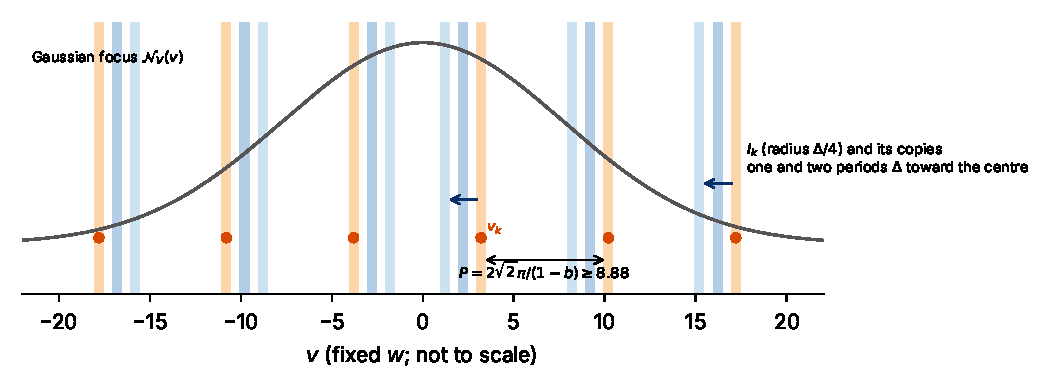
\includegraphics[width=\columnwidth]{figures/fig_lemma7.pdf}
\caption{Schematic of the proof of Lemma~\ref{lem:P} (not to scale). For fixed $w$ the phase mismatch $\phi$ vanishes only near the points $v_k$ (dots), which are $P\ge8.88$ apart. Outside the intervals $I_k$ of radius $\Delta/4$ (shaded), $\phi$ is bounded below. The weight $q=\mathcal N_V h s_v^2$ inside $I_k$ reappears one and two periods $\Delta$ closer to the centre of the focus (arrows), where $\phi$ is not small; the Gaussian focus (curve) costs at most the factor $e^{-10\pi^2/\tau}$.}
\label{fig:lemma7}
\end{figure}

\begin{proof}[Proof of Lemma~\ref{lem:P}]
If $b\ge1$ the bracket vanishes, $c_P=0$, and the claim $N_\phi\ge0$ is clear because the integrand is non-negative. Let $0<b<1$.

We have $N_\phi=(\sigma^2/2)\iint p\,s_v^2\phi$, $\phi=1-\cos m_z\ge0$, $\sqrt2m_z=v+\sigma^2s_v+w+\sigma^2s_w$, with $s_v=-v/V+k'h_t/h$ and $s_w=(\ln\Gamma)'(w)+h_w/h$ ($=-w/L^2+h_w/h$ for $\Gamma=N(0,L^2)$).
The integrand is non-negative.

\emph{The phase.}
Since $\sigma^2s_v=-bv+\sigma\sqrt x\,h_t/h$,
\begin{gather}
\sqrt2m_z=(1-b)v+c(w)+\varepsilon(v,w),\nonumber\\ c(w)=w+\sigma^2(\ln\Gamma)'(w),\qquad \varepsilon=\sigma\sqrt x\frac{h_t}h+\sigma^2\frac{h_w}h .
\end{gather}
The proof uses about $\Gamma$ only that, for fixed $w$, $c(w)$ is a number independent of $v$.
Since $|\sigma\sqrt xh_t/h|\le\sigma\sqrt xN_1/(1-\Qb)$ and $|\sigma^2h_w/h|\le\sigma^2(|w|/s^2)e^{-w^2/2s^2}\Qb/(1-\Qb)\le\sigma\Qb e^{-1/2}/(1-\Qb)$ (using $s\ge\sigma$), we have $|\varepsilon|\le\sigma a$.

\emph{Fix $w$.}
Let $v_k=(2\sqrt2\pi k-c(w))/(1-b)$, $k\in\mathbb Z$, $r=\Delta/4$, $I_k=(v_k-r,v_k+r)$ and $I=\bigcup_kI_k$.
The spacing is $P=2\sqrt2\pi/(1-b)\ge2\sqrt2\pi>8.88$ because $0<1-b<1$.

\emph{(i) Outside $I$, $\phi$ is bounded below.}
For $v\notin I$ the distance of $(1-b)v+c(w)$ to $2\sqrt2\pi\mathbb Z$ is at least $(1-b)r$, so the distance of $m_z$ to $2\pi\mathbb Z$ is at least $((1-b)r-\sigma a)_+/\sqrt2$.
With $1-\cos u\ge2u^2/\pi^2$ on $|u|\le\pi$,
\begin{equation}
\phi\ \ge\ \phi_r=\frac{((1-b)r-\sigma a)_+^2}{\pi^2}=\frac{\sigma^2}{4x}\Bigl((1-b)-\frac{2a\sqrt x}\pi\Bigr)_+^2 .
\end{equation}

\emph{(ii) The weight inside $I$ is also outside.}
Let $q(v)=\mathcal N_V(v)h(k'v,w)s_v(v,w)^2\ge0$.
Fix $k$, let $\epsilon_k=\mathrm{sgn}(v_k)$ ($+1$ if $v_k=0$), $v\in I_k$, and $u_j=v-j\epsilon_k\Delta$, $j=1,2$: one and two periods towards the centre of the focus.
Because $h$ and $h_t$ have period $2\pi$ in $t=k'v$ and $k'\Delta=2\pi$, they take the same values at $u_j$ and at $v$, while $s_v(u_j)=s_v(v)+jd$, $d=\epsilon_k\Delta/V$.
The Gaussian ratio is $\mathcal N_V(u_j)/\mathcal N_V(v)=\exp(j\Delta(2\epsilon_kv-j\Delta)/(2V))$; since $\epsilon_kv\ge|v_k|-r\ge-\Delta/4$, the exponent is at least $-j(j+\tfrac12)\Delta^2/(2V)\ge-\tfrac52\Delta^2/V=-10\pi^2/\tau$ for $j\le2$ (because $\Delta^2/V=4\pi^2/\tau$).
Moreover $(s+d)^2+(s+2d)^2\ge s^2/5$ for all $d$ (the minimum is at $d=-3s/5$).
Hence $q(u_1)+q(u_2)\ge e^{-10\pi^2/\tau}q(v)/5=\theta q(v)$, and integrating over $v\in I_k$,
\begin{equation}
\int_{I_k-\epsilon_k\Delta}q+\int_{I_k-2\epsilon_k\Delta}q\ \ge\ \theta\int_{I_k}q .
\end{equation}
The shifted intervals have centres at distance $\Delta$ and $2\Delta$ from $v_k$ and radius $\Delta/4$; they are disjoint from each other and from $I_k$.
All lie within $2\Delta+\Delta/4$ of $v_k$, and $2(2\Delta+\Delta/4)=4.5\Delta<8.88\le P$ for $\Delta\le1$, so they meet no other $I_{k'}$ and no shifted interval of another $k$ (whatever its direction).
All lie outside $I$.
Summing over $k$: $\int_{I^c}q\ge\theta\int_Iq$, that is $\int_{I^c}q\ge\frac\theta{1+\theta}\int q$.

\emph{Conclusion.}
$\int q\phi\,dv\ge\phi_r\int_{I^c}q\ge\phi_r\frac\theta{1+\theta}\int q\,dv$.
Multiplying by $\Gamma(w)/Z$ and integrating over $w$ gives $\E[s_v^2\phi]\ge\phi_r\frac\theta{1+\theta}\Jvv$, so
$N_\phi\ge\frac{\sigma^2}{8x}\frac\theta{1+\theta}((1-b)-2a\sqrt x/\pi)_+^2\,\sigma^2\Jvv$, and $\sigma^2\Jvv=b+W$ by Lemma~22 of~\cite{F}.
\end{proof}

The constant is loose on purpose.
The true $N_\phi/(b+W)$ is of size $1/(8B)$ \numst, and $c_P$ is smaller than that by about $\tau$; the law needs only the size $\sigma$.
In the class, $\Delta\le2\pi/\sqrt{5\times10^{11}}<10^{-5}$, far inside the condition $\Delta\le1$.
Moving the weight three or more periods may improve $\theta$, at the price of a stronger disjointness condition and a faster Gaussian decay; the theorem does not need it, and we have not tried.

\emph{Picture.}
Over hundreds of periods the observer no longer sees single ripples but their average brightness.
The information that reaches her is the slope information of the ripple times the phase mismatch between the centre and the edge of the focus, and the mismatch is as large as the focus is wide: the information is of size $1/(B\sigma)$, which exceeds what the law asks by a factor of order $e^\ell$.
The cross term between curvature and mismatch, measured over the whole ripple rather than at its worst point, takes $8\%$ of it.
When the focus spans only a few periods the average is not available, but the ripple repeats.
A steep slope hidden where the mismatch happens to vanish is present again one period and two periods away, where it does not vanish; it is dimmer there, in the tail of the focus, but brightness is never negative, so it is only discounted, never cancelled.
